\chapter{Theory of atomistic representations}
%\markboth{Theory of atomistic representations}{Theory of atomistic representations}
%\addcontentsline{toc}{chapter}{Theory of atomistic representations}
\label{sec:atomistic_representation}

Physical properties, such as energies, dipole moments and polarizabilities, all exhibit symmetries that can be exploited to facilitate the construction of a surrogate model that learns a relationship to such properties from geometric information.
By embedding the symmetries into the numerical description of the atomic structure the hypothesis space is reduced that needs to be considered by the learning algorithm, thereby resulting in more effective models.
This chapter covers the theory and computation of symmetrized features on the atomic-scale.
%The methods presented have been historically developped incrementally improving fferent aspects in the computation of the 
%advantage of mathematical tricks to compute efficiently features, the connection between those has been much later.
%We take an approach similar to ~\cite{willatt2019atom} defining summarizing all approaches 
A similar approach as in Ref.~\cite{will+19jcp} is taken that introduces the topic by utilizing concepts from representation theory to give a more profound understanding of the approaches existing in the field.
We therefore begin with introducing the representation $f_A:\Omega\rightarrow\mathbb{R}$ of an atomic structure $A$ on a smooth manifold $\Omega\subseteq\mathbb{R}^{z}$, where we use $\Omega$ to consider different encodings of the atomic structure $A$.
%We will refer to these different encondings as \emph{featurizations}, which
In its simplest form, an encoding can be the atomic positions $\mathbf{q}\in\mathbb{R}^{3N}$ of structure $A$.
To construct a numerical description for a structure $A$ that can be used as input for a data-driven model, we project on its representation with an orthonormal set of \emph{basis functions} $\{b_k:\Omega\rightarrow\mathbb{R}\}_{k=1}^{M}$, to obtain a set of \emph{expansion coefficients} $\{c_k\in\mathbb{R}\}_{k=1}^{M}$ from the basis expansion
\begin{equation}
  c_k = \int_\Omega\mathrm{d}\mathbf{x}\,\, f_A(\mathbf{x})b_k(\mathbf{x})\text{ for }k=1,\ldots M.
\end{equation}
For a lot of cases the orthonormality constraint of the basis is relaxed, since the orthonormalization can be seen as part of the learning algorithm.
%Even though pre-orthonormalization has an effect on the regularization term, often found in shallow models, 
%Then we project these functions on the representation, 
%that can be used to build a model mapping the coefficients to phyisical properties like energy and forces.
The choice of the representation space as well as the basis is essential for an effective numerical description, i.e. a description that captures information with fewer number of coefficients. 
We will refer to the whole process of transforming a structure $A$ to a representation and then to a numerical description as \emph{featurization} of structure $A$ as depicted in Figure~\ref{fig:acdc-scheme}.
%The advantage of such a mathematical rigorous approach is a clearer understanding of the target we 
%For an orthonormal basis we in the limit of basis functions
%\begin{equation}
%  \sum_k c_k b_k(\mathbf{q}) = f(\mathbf{q})
%\end{equation}
A widely-used family of representation spaces is based on higher orders of atom-density-based functions.
This family of representation spaces is introduced and it is shown how invariances can be efficiently embedded into the computation of the expansion coefficients.
%Prior knowledge about physical properties and distributions of atomic structures is therefore used to bias the functional form and basis functions to produce more effective coefficients~\cite{behl11jcp,drautz2019atomic}.
%Some of the bias are presented here.
%\emph{atom-centered density correlation} (ACDC) function representing the atomic structure as correlation between local atomic densities is introduced and its connection to widely established descriptors is shown.
Additionally, general characteristics of basis functions deployed in atomic-scale models are presented as well as different practices to transform the expansion coefficients into inputs for data-driven models.
 
% and how to efficiently embed invariances into these are presented.
\begin{figure}
  \centering
  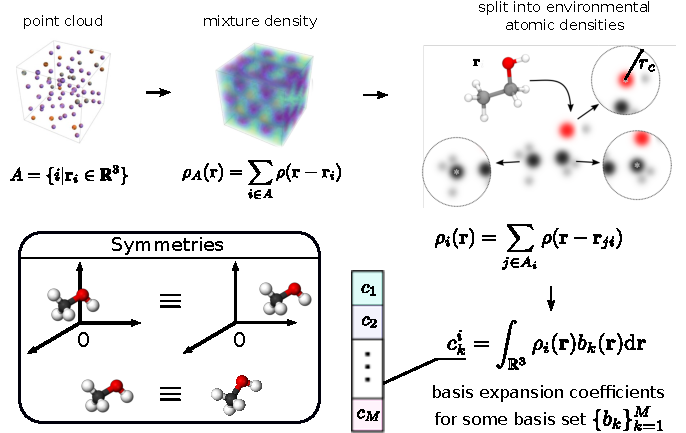
\includegraphics[width=\textwidth]{fig/atomistic_repr_schematic.pdf}
  \caption{A schematic showing the featurization of an atomic structure $A$ based on the atom-centered density correlations functions. The figure of the atoms in the box are retrieved from Ref.~\cite{noh2019inverse}. The figure of the atomic environments is retrieved from Ref.~\cite{will+19jcp}. The methanol molecule is retrieved from Ref.~\cite{wiki:Alcohol_(chemistry)}.}
  \label{fig:acdc-scheme}
\end{figure}

%In the following methods of encoding the information present in the symmetrized many-body correlation function in Eq.~\eqref{eq:invariant_many_body_correlation_function} into a vector representation are presented.

%By separating the atomic structure descriptor into descriptors for atomic environments different methods for constructing a structural descriptor out of atomic environment contributions have been proposed.

%% add maybe the fingerprint in zhu2016fingerprint based on local overlap matrix
\section{Atom-centered density}
\label{sec:environment}
%Based on the successfully used assumption that the atomic nuclei can be
%treated classically, we can directly use the geometric information of the
%atomic nuclei.  and  used in Born-Oppenheimer and Car-Parinello molecular
%dynamics simulation Breaking down atomic structure wavefunction into atomic
%positions is rationalized by the Born-Oppenheimer approximation treating
%nuclear and electron wavefunction separately due to their large difference in
%mass.
%% TODO read the KS paper again, there should be a reasoning for the atomic structure potential to the energy
%Another assumption done in Born-Oppenheimer and Car-Parinello molecular
%dynamics is to treat the nucleus classical, thus the a full representation of
%the atomic structure by the positions of its nuclei and their chemical species
%exist.  Furthermore, in contrast to the previous approach, a continuous
%function exists mapping the positions of the atoms to a physical property of
%the atomic structure.
%%Furthermore, the nuclei and treating the nuclei classically, the atomic structure can be fully represented by the positions of its nuclei and their chemical species.
%%Furthermore, in this framework a continuous function exists mapping these information to a physical property.
%As a consequence efficient encapsulation of geometric information of atomic
%structures into a descriptor has dominated recent development of descriptors
%in the atomic scale~\cite{willatt2019atom}.  TODO maybe Within the
%Car-Parinello framework
%To this end several methods have been proposed to incorporate into a descriptor transformations under which the target atomic properties are equivariant~\cite{willatt2019atom}.
%%and for models~\cite{schutt2018schnet} have been proposed.
%For scalar properties, these transformations are rotations and translations of
%the atomic structure, and permutations of the atom order.  From a statistical
%learning theory perspective the incorporation of invariances into the
%descriptor can be seen as a reduction of the hypothesis class in size
%% and in the model case as the introduction of prior knowledge into the model.
%~\cite{willatt2019atom}.
A majority of developed atomistic descriptors can be seen as different approaches to construct the expansion coefficients based on a family of functions, that originates from the structural density function~\cite{musil2021physics} 
\begin{equation}
  \label{eq:basis_expansion}
  \sum_{i\in A} \rho(\mathbf{r}-\mathbf{r}_i)\text{ for an atomic density }\rho:\mathbb{R}^3\rightarrow\mathbb{R},
\end{equation}
where $\mathbf{r}_i\in\mathbb{R}^3$ is the position of the $i$th atom in the atomic structure $A$ and $\rho$ is an arbitrary function decaying from its origin. 
Commonly, a Gaussian $g$ or a Dirac $\delta$ function are chosen as atomic density $\rho$.
A widely adapted approach to impose translational invariance, i.e. independence of the center of the structure, is to describe the atomic structure as a sum of atomic environment contributions, each of them defined as a sum over the densities in their corresponding neighborhood
\begin{subequations}
\begin{align}
  \rho_{ij}(\mathbf{r}) &= \rho(\mathbf{r}-\mathbf{r}_{ji}),\quad \rho_{ij}:\mathbb{R}^3\rightarrow\mathbb{R}\quad\text{(neighbor density of atom $j$ centered at $i$)},
  \label{eq:neighbor_density} \\
  \rho_i(\mathbf{r}) &= \sum_{j\in A_i} \rho_{ij}(\mathbf{r}),\quad \rho_i:\mathbb{R}^3\rightarrow\mathbb{R}\quad\text{(environmental density of atom $i$)},
  \label{eq:density_atomic_contributions}
\end{align}
\end{subequations}
where $A_i$ is the set of all atoms that are in the \emph{environment} of atom
$i$, in most applications defined as the set of atoms within a certain distance, the
\emph{cutoff}, and $\mathbf{r}_{ji}$ is the direction vector $\mathbf{r}_j-\mathbf{r}_i$. 
While we refer to $\rho_i$ as environmental density in this thesis, the term atomic density is however frequently more loosely used to refer also to $\rho$ centered at position $i$~\cite{musil2021physics}.
This approach further aligns with the partitioning of a structure property $y_A$ into local atomic contributions
\begin{equation}
  \label{eq:structural_separation}
  \sum_{i\in A} y_i = y_A
\end{equation}
which is motivated by the heuristical observation that atomic properties decay with their distance to the center, a concept commonly referred to as \emph{locality} or \emph{nearsightedness}~\cite{prodan2005nearsightedness}.
%The exact meaning of this atomic contributions is still a reasearch question.
\section{Hierarchy of invariant representations}
%tensorial properties
%Learning tensorial properties requires change under rotation~\cite{chemrev}.
%Cartesian tensors can be transformed to this basis using a set of rules~\cite{cartesiantransformationTODO}
%Such equivariant behavior under rotation can be embedded by splitting the density function over the corresponding SO(3) subgroup.
%It is required to increase the higher-body orders and predicting tensorial properties to separate the density function into its irreducible spherical tensors 
%\begin{equation}
%\label{eq:integration_over_subgroup}
%%\ket{A^{(n)}}_{\hat{R}\hat{t}} = \int \mathrm{d}\hat{R}\,\int \mathrm{d}\hat{t}\, \bigotimes_{m=1}^n\hat{R}\hat{t}\ket{\mathcal{A}}
%  \ket{\mathcal{X}^{(\nu)}}_{\hat{R},h} = \int_{SO(3)} \hspace{-1em}\mathrm{d}\hat{R}\, \underbrace{\hat{R}\ket{\mathcal{X}}_h\otimes \cdots \otimes \hat{R}\ket{\mathcal{X}}_h}_{\nu-\text{times}}, %TODO change equation
%\end{equation}
As a large family of physical quantities are invariant under rotations of the atomic structure, it is thus required to account for rotational invariance in the process of relating atomic structures to such quantities.
Rotational invariance can be embedded into the representation by simply introducing a Haar integral over the rotation group $SO(3)$
\begin{equation}
\label{eq:integration_over_subgroup}
\overline{\rho_i^{\otimes 1}}(\mathbf{r}) = \int_{SO(3)}\mathrm{d}\hat{R}\, \rho_i(\hat{R}\mathbf{r})\quad\textrm{(ACDC of order 1)}
\end{equation}
which can be further extended to higher-order correlations of the density
\begin{equation}
\label{eq:integration_over_subgroup_higher_order}
\overline{\rho_i^{\otimes\nu}}(\mathbf{r}^{(1)},\ldots, \mathbf{r}^{(\nu)}) = \int_{SO(3)}\mathrm{d}\hat{R}\, \rho_i(\hat{R}\mathbf{r}^{(1)})\ldots\rho_i(\hat{R}\mathbf{r}^{(\nu)})\quad\textrm{(ACDC of order $\nu$)}.
\end{equation}
This class of representations has been named \emph{atom-centered density correlations} (ACDC) functions~\cite{nigam2022unified}.
Although it is theoretically possible to evaluate this integral numerically, it does not offer an efficient means to determine the expansion coefficients.
Hence, it is essential to choose suitable candidates for the density $\rho$ and the basis set $\{b_k\}_{k=1}^M$ that yield an efficient solution for the integral.
%Note that post-symmetrization methods have recently been developed that also allow an efficient evaluation of the integral by averaging over all possible reference frames within a order $\nu$ tuple~\cite{pozdnyakov2023smooth}, these are however not in the scope of the thesis.

\subsection{Solution for Dirac $\delta$ densities}

%It has been shown that most representations can be derived naturally from atomic density by constructing higher-order correlations and imposing rotational invariance~\cite{willatt2019atom}.
%Rotational invariance is obtained by taking the Haar integral of the function over the $SO(3)$ group, i.e. integrating over all 3D rotations.
An explicit solution of the integral over $SO(3)$ can be expressed for the Dirac $\delta$ densities.
Here we present the solutions for order 1 and 2 
\begin{subequations}
\label{eq:dirac_delta_haar_integral}
\begin{align}
    \label{eq:dirac_delta_haar_integral_2body}
    \sum_j \int_{SO(3)} \mathrm{d}\hat{R}\, \delta(\hat{R}\mathbf{r}-\mathbf{r}_{ji}) &\propto_r \sum_j \delta(r-r_{ji})\quad\textrm{(order 1)},  \\% = f^1(r)\\
    %\langle r| \mathcal{X}_i\rangle_{\hat{R},g\rightarrow\delta} &\propto \sum_{j\in\mathcal{X}_i}\delta(r-r_{ij}), \\
    \label{eq:dirac_delta_haar_integral_3body}
    %\langle rr'\theta | \mathcal{X}^{(2)}_i\rangle_{\hat{R},g\rightarrow\delta} &\propto \sum_{j,k\in\mathcal{X}_i} \delta(r-r_{ij})\delta(r-r_{ik})\delta(\theta-\theta_{ijk}),
    \sum_{jk}\int_{SO(3)} \mathrm{d}\hat{R}\, \delta(\hat{R}\mathbf{r}-\mathbf{r}_{ji}) \delta(\hat{R}\mathbf{r}^\prime-\mathbf{r}_{ki}) &\propto_r \sum_{jk}\delta(r-r_{ji})\delta(r^\prime-r_{ki})\delta(\theta -\theta_{jki})\quad\textrm{(order 2)}, %= f^2(r, r, \theta)
    %\delta(r^\prime-r_{ki})\delta(\theta-\theta_{jki}). %= f^2(r, r, \theta)
\end{align}
\end{subequations}
where we use $\mathbf{r}$ and $\mathbf{r}^\prime$ as shorter notation to refer to $\mathbf{r}^{(1)}$ and $\mathbf{r}^{(2)}$.
%that should make clear how it generalizes to higher orders.
We use $\propto_r$ to omit constant factors and radial terms $r$ that appear due to the integration over the rotation group.
These factors are not essential, since typically a radial scaling term is added to the density to control the general scaling~\cite{behl11jcp,huan-vonl16jcp,will+18pccp,drautz2019atomic}.
The correlation function of order 1 naturally results in a description of the distance to atom $i$ and the order 2 function in the two distances and an angle with respect to atom $i$.
This can be generalized to higher orders retrieving a decomposition into different body-order contributions as it is done for interatomic potentials.
This expansion makes the close relationship clear between ACDC-based descriptors to interatomic potentials that decompose the energy into different body-order contributions.
%\begin{multline}
%  f^\nu(\mathbf{r}_1,\ldots, \mathbf{r}_\nu) \proto_r f^\nu(\mathbf{r}_1,\ldots, \mathbf{r}_\nu)\delta(r-r_{ij_1})\ldots\delta(r-r_{ij_\nu})
%  \delta(r-r_{j_1j_2})\ldots\delta(r-r_{j_1j_\nu})\ldots\delta(r-r_{j_2j_3})\ldots\delta(r-r_{j_2j_\nu})\ldots\delta(r-r_{j_{\nu-1}j_\nu})
%\end{multline}

\subsection{Ordered support of representation}
%from the representation is to use its supportto obtain a numerical input 
One early-developed approach to obtain a numerical input has been to directly use the discrete many-body information (e.g. 2-body distances in the environment) in form of a concatenated vector.
The vector is then sorted to achieve permutational invariance~\cite{hansen2015machine, barker2016localized, huang2016communication}.
%, (e.g. 2-body distances in Refs.~\cite{rupp2012fast, montavon2012learning, montavon2013machine, sadeghi2013metrics} or 3-body angles and 4-body torsions in Ref.~\cite{huang2016communication}).
%The discrete $(\nu-1)$-body information is then sorted~\cite{hansen2015machine, barker2016localized, huang2016communication}. % or averaged over numerous random permutations~\cite{montavon2012learning, montavon2013machine, sadeghi2013metrics} to embedd permutational invariance into the description.
The sorting of the many-body information approach can be connected to the ACDC descriptors by a change of the metric space from the $L^1$ norm distance to the earth mover's distance (EMD)~\cite{will+19jcp}.
The relationship can be clearly seen by using the fact that the EMD between two distributions $\textrm{p}$ and $\textrm{p}^\prime$ can be connected to the $L^1$ distance between the inverses of the cumulative density functions $P$ and $P^\prime$ of those distributions
\begin{equation}
  \label{eq:emd_lp_duality}
  \operatorname{EMD}(\textrm{p}, \textrm{p}^\prime)=\int_0^1\mathrm{d}{s}\,\left|P^{-1}(s) -{P^{\prime}}^{-1}(s)\right|\text{, with }P(x)=\int_{-\infty}^s \mathrm{d}x\, \textrm{p}(x).
\end{equation}
Then the EMD between two order 1 ACDC functions using the Dirac $\delta$ function as atomic density is equal up to a normalization factor dependent on the number of atoms to the $L^1$ difference between their sorted distances vectors~\cite{will+19jcp}.
%\begin{subequations}
%  \begin{align}
%    \|R_A-R_B\| = $\overline{\rho^{\otimes}}$
%    [R]_{ji} = r_{ji}
%  \end{align}
%\end{subequations}
%As a consequence there exists a one-to-one mapping between t
%As a consequence the EMD between two order 1 ACDC functions based on Dirac $\delta$ densities is corresponds to the absolute distance between the two sorted distances corresponding to the same environments up to a global normalization factor.
This fact can be extended to the $L^p$ norm distance denoted by the term $W_p$ referring to the more common naming \emph{Wasserstein distance} for the EMD.
\begin{equation}
  \label{eq:emd_lp_duality}
  W_p(\textrm{p}, \textrm{p}^\prime)^p=\int_0^1\mathrm{d}{s}\,\left|P^{-1}(s) -{P^{\prime}}^{-1}(s)\right|^p.
\end{equation}
%Another existential crisis is that the Wassertstein distance is usually applied for robustenss, we dont need robustness
It is not clear how the Wasserstein metric applied to higher orders of the ACDC functions changes the nature of the representation, since for higher dimensions a form as in Eq.~\eqref{eq:emd_lp_duality}, reproducing the Wasserstein distance by the $L^p$ distance for a representation, is not known.
%In addition to this problem, there is also no unique mapping from a distance metric to a similarity measure.
%For example, from the $W_2$ metric we the normalized sorted distance vectors can be formulated $\mathbf{s}\cdot \mathbf{s}^\prime$ and $\exp(\|\mathbf{s}-\mathbf{s}^\prime\|^2)$ valid similarity measure, as defined in Ref.~\cite{app11041910}. 
An approach that extends this idea to higher orders utilizes sorted angles or sorted torsions as description~\cite{huang2016communication}.
These can be seen as one-dimensional projections of the higher-order ACDC functions and do not consider the whole coherent space of correlations.
It has been shown that descriptors in this category can reach comparable accuracies to the common methods that can be induced from the Euclidean metric~\cite{barker2016localized,huang2016communication} with energy accuracies close to 1 kcal/mol on the QM9 and QM7b dataset. % as well as an efficient removal of the discontinuouties introduced by the sorting as well as 
These descriptions nevertheless have undesired characteristics with regard to differentiability and extensibility.
The sorted quantities have discontinuities with respect to changes in the atomic positions that emerge when two distances are swapped due to the sorting, which is problematic for predictions of derivatives.
These discontinuities can however be mitigated by smoothing the descriptor within a similarity or distance measure.
Another problem is that their size depends on the number of atoms in the local environment being represented, thus they are often padded with zero values impeding their application to neighborhoods with diverse number of atoms.

%the discontinuities introduced by the rearrangement still remains a problem that makes them unsuitable candidate for interatomic potentials.
%For global structural descriptors the 2-body distances is often put into a matrix form to then utilize the sorted eigenvalues as descriptor~\cite{rupp2012fast, sadeghi2013metrics, zhu2016fingerprint}.
%For that the discrete $(\nu-1)$-body information is even directly used sorted vector~\cite{hansen2015machine, barker2016localized, huang2016communication} or put into a matrix form to then utilize its sorted eigenvalues as descriptor~\cite{rupp2012fast, sadeghi2013metrics, zhu2016fingerprint}, or 

%and then further rearrantransformed to embedd permutational invariance into the description.
%This canonical or utilizing the sorted eigenvalues~\cite{rupp2012fast, sadeghi2013metrics, zhu2016fingerprint} or the sorted $\nu$-tensor entries~\cite{hansen2015machine, barker2016localized, huang2016communication}.
%For the 2-body distances it has been shown that these two approaches introduce degeneracies, i.e. points that map different atomic structures to the same descriptor~\cite{moussa2012comment}.
%A solution to avoid these degeneracies has been to sum over random permutations of the matrix~\cite{montavon2012learning, montavon2013machine, sadeghi2013metrics}.
%While this approach can be applied for small molecules, it does not scale well with the number of atoms.
%A still computational very costly but feasible solution is to find a canonical permutation for all environments in the data set by constructing a transitive closure of all bi-partite permutations~\cite{chmiela2018towards}.
%The bi-partite permutations are determined by solving the matching problem between the principal eigenvectors of two matrices with the Hungarian algorithm~\cite{kuhn1955hungarian}, the transitive closure is constructed with a minimum spanning tree.
%Even though, the degenaricies it has been shown for several regression tasks that descriptors in this category can reach high accuracies~\cite{barker2016localized,huang2016communication}, the discontinuity introduced by arranging them in a permutative invariant manner still remains a problem that makes them unsuitable candidate for interatomic potentials.
%
%-o a vectorial form by concatenating the discrete information into n

%In the view of the ACDC funciont is the support of the of the ACDC functions with Dirac $\delta$ distributions.
%, the values of the function that do not evaluate to zero, and concatenate the information to a tensorial form.
%These approaches introduce permutational into the tensorial form in different manners,  
%In the case of the order 1 function as described in Eq.~\eqref{eq:dirac_delta_haar_integral_2body} it corresponds to the 2-body distances $r_{ji}$ of an evironment.
%In the view of basis expansion coefficients this approach can be seen as selecting a different basis set of Dirac $\delta$ functions for each atomic environment.
%These  values are then concatenated into a vectorial form by construct

%For example, the 2-body distances $r_{ji}$ can be derived from the order 1 Eq.~\eqref{eq:dirac_delta_haar_integral_2body} by chosing for each atomic environment $i$ the basis set $\{\delta(r-r_{ji}):\mathbb{R}\rightarrow\mathbb{R}\}_{j\in A_i}$.
%
%We can for example derive the 2-body
%
%Since the number of distances changes through the environments the cona
%The problem is to converge this to an 
%
%Another approach is to interpret the as a different
%
%Since the number of distances 
%The method to put this in a set of coefficients that can
%
%
%This is however also where ca

%%\begin{equation}
%%[f(\ket{\mathcal{A}\otimes\mathcal{A}\rangle},\ket{\mathcal{A}\otimes\mathcal{A}\rangle})]_{ij}
%%% can generalized to environments
%%\end{equation}
%%\begin{equation}
%%    C_{ij} = \langle r_i r_j|\mathcal{X}^{(n)}\rangle
%%    \langle r_1\ldots r_{n^2}|\mathcal{X}^{(n)}\rangle
%%\end{equation}
%To achieve permutational invariance the sorted eigenvalues~\cite{rupp2012fast, sadeghi2013metrics, zhu2016fingerprint} or sorted tensor entries~\cite{hansen2015machine, barker2016localized, huang2016communication} have been used as descriptor.
%For the pairwise distances it has been shown that both approaches for permutational invariance suffer from degeneracies, mapping different atomic structure to the same descriptor~\cite{moussa2012comment}.
%A solution to avoid these degeneracies has been to sum over random permutations of the matrix~\cite{montavon2012learning, montavon2013machine, sadeghi2013metrics}.
%While this approach can be applied for small molecules, it does not scale well with the number of atoms.
%A still computational very costly but feasible solution is to find a canonical permutation for all environments in the data set by constructing a transitive closure of all bi-partite permutations~\cite{chmiela2018towards}. The bi-partite permutations are determined by solving the matching problem between the principal eigenvectors of two matrices with the Hungarian algorithm~\cite{kuhn1955hungarian}, the transitive closure is constructed with a minimum spanning tree.
%Although it has been shown for several regression tasks that descriptors based on this approach can reach high accuracies~\cite{barker2016localized,huang2016communication}, the discontinuity introduced by arranging them in a permutative invariant manner still remains a problem that makes them unsuitable candidate for interatomic potentials.

%local atomic environment version of the sorted pairwise distances matrix~\cite{barker2016localized} and a sorted 4-body torsion tensor~\cite{huang2016communication} can reach accuracies comparable with descriptors using the branch of approaches we introduce in the next section.
%
%h it has been shown that for several regression tasks that a local atomic environment version of the sorted pairwise distances matrix~\cite{barker2016localized} and a sorted 4-body torsion tensor~\cite{huang2016communication} can reach accuracies comparable with descriptors using the branch of approaches we introduce in the next section.
%
%Although the regression performance of descriptors based on this approach is comparable ~\cite{barker2016localized,huang2016communication} to the descriptors based on the approach we introduce in the next section, the discontinuity seems
%In the next section we introduce a branch that leads to more accurate results~\cite{de2016comparing, bartok2017machine, jager2018machine}, 

\subsection{Fixed basis set}
%%\[\langle\mathbf{r}\mathbf{r'}|{\mathcal{A}\otimes\mathcal{A}}\rangle = \sum_i g(\mathbf{r}-\mathbf{r}_{ij})\]
%The use of projections of the symmetrized many-body correlation function has been one of the early ways to construct a descriptor.
%As the sorted support leads to a discontinuous description, a solution that does not 
Considering the order 1 solution in Eq.~\eqref{eq:dirac_delta_haar_integral_2body} with an additional radial factor $r$
%density using Dirac $\delta$ densities
\begin{equation}
  f(r) = r \sum_j \delta(r-r_{ji}),  % = f^1(r)\\
\end{equation}
we can retrieve the 2-body distances used for sorted distance by using a basis set of the form $\{\delta(r-r_{ji}):\mathbb{R}\rightarrow\mathbb{R}\}_{j\in A_i}$ with a subsequent sorting.
From this point of view the cause of the discontinuities exihibited by the descriptors in the last section can be attributed to the variation of the basis function across atomic environments.
A natural solution is therefore the usage of the same basis set across all environments in all structures~\cite{behl11jcp,bart+13prb,drautz2019atomic}.
By expanding on the ACDC function using the Dirac $\delta$ function for the densities with the basis functions $\{b^\nu_k\}_k$ of different orders one obtains coefficients of the form
\begin{subequations}
\label{eq:dirac_delta_expansion_coeffs}
\begin{align}
    \label{eq:dirac_delta_expansion_coeffs_2body}
    \int_{\mathbb{R}^3}\mathrm{d}\mathbf{r}\, b^1_k(r)\delta(r-r_{ji}) &\propto_r b^1_k(r_{ji}),\\
    \label{eq:dirac_delta_expansion_coeffs_3body}
    \int_{\mathbb{R}^3\times\mathbb{R}^3}\mathrm{d}\mathbf{r}\mathrm{d}\mathbf{r}^\prime\, b^2_k(r,r\prime,\theta(\mathbf{r}\cdot\mathbf{r}^\prime))\delta(r^\prime-r_{ji})\delta(r-r_{ki})
    \delta(\theta(\mathbf{r}\cdot\mathbf{r}^\prime) - \theta_{jki}) &\propto_r b^2_k(r_{ji},r_{ki},\theta_{ijk}).
    %\delta(\hat{\mathbf{r}}\cdot\hat{\mathbf{r}}^\prime - \hat{\mathbf{r}}_{ji}\cdot\hat{\mathbf{r}}_{ki})
\end{align}
\end{subequations}
One widely-used representative of this approach is the Behler-Parrinello symmetry function (BPSF)~\cite{behl11jcp}.
In the next section we discuss how this approach is extended for Gaussian densities. 

\subsection{Radial and angular decomposition}
%to obtain a continuous description~\cite{behlerparinello}.
%As example two types of basis functions the atom-centered symmetry functions (ACSFs)~\cite{behl11jcp}
%The main characteristics of the these functions can be seen in the following examples
%
%\begin{subequations}
%\begin{align}
%G_2(r) &=  \exp(\eta(r-r_s)^2), \\
%%original form
%%G_4(\theta, \mathbf{r}) &= 2^{1-\eta} (1+\lambda \cos(\theta))^{\zeta} \exp(-\eta\|\mathbf{r}\|^2),
%G_4(r, r',\theta) &= 2^{1-\zeta} (1+\lambda \cos(\theta))^{\zeta} \exp(-2\eta(r^2+r'^2 -rr'\cos(\theta))),
%\end{align}
%\end{subequations}
%where $r_s$, $\lambda,\zeta$ and $\eta$ are parameters which are chosen \textit{a priori} computation.
%The expansion coefficients are computed by expanding on the Diral $\delta$ density
%\begin{subequations}
%  \label{eq:symmetry_function_as_projection}
%  \begin{align}
%    %\langle G_2|\mathcal{X}_i\rangle_{\hat{R},g\rightarrow\delta} &= \sum_{j\in\mathcal{X}_i} G_2(r_{ij})\\
%    \int G_2(r)\delta(r-r_{ij}) \,\mathrm{d}\mathbf{r} &\propto G_2(r_{ij})\\
%    %\langle G_4|\mathcal{X}_i^{(2)}\rangle_{\hat{R},g\rightarrow\delta} &= \sum_{j,k\in\mathcal{X}_i} G_4(r_{ij},r_{ik}, \theta_{ijk}),
%    \int G_4(r,r\prime,\theta_{ijk})\delta(r-r_{ij})\delta(r-r_{ik})\delta(\theta-\theta_{ijk}) \,\mathrm{d}\mathbf{r}\mathrm{d}\mathbf{r}^\prime &\propto G_4(r_{ij},r_{ik}, \theta_{ijk})
%  \end{align}
%\end{subequations}
For Gaussian densities the order 1 expression in Eq.~\eqref{eq:integration_over_subgroup} can be analytically solved by exploiting properties of the Gaussian function~\cite{musil2019machine}
\begin{subequations}
\begin{align}
  \label{eq:order1_analytical_solution}
  \int_{SO(3)} \mathrm{d}\hat{R}\, g(\hat{R}\mathbf{r}-\mathbf{r}_{ji}) %\propto_r ... \approx g(r-r_i) 
   &= \int_{SO(3)} \mathrm{d}\hat{R}\, \exp(\|\hat{R}\mathbf{r}-\mathbf{r}_{ji}\|^2/(2\sigma^2)) \\
   &= 8\pi^2 \sinh(rr_{ji}^2/2\sigma^2)(rr_{ji}/2\sigma^2)\exp(-(r^2+r_{ji}^2)/4\sigma^2) \\
   &\approx \frac{1}{r_{ij}}\exp(-((r-r_{ji})^2)/4\sigma^2)
\end{align}
\end{subequations}
which gives approximately a Gaussian density in radial space.
%An expansion for er density functions requires results from angular momentum theory to solve the integral.
A solution of the integral for higher orders requires a more complex derivation utilizing mathematical properties of spherical harmonics $Y_m^l(\hat{\mathbf{r}}):S^2\rightarrow\mathbb{R}$. % from angular momentum theory~\cite{yutsis1965theory}.
%egral s usually solved by expressing the density as a product of a radial and angular function
%\begin{equation}
%  \label{eq:radial_angular_density}
%  \rho(\mathbf{r}) = \rho_r(r)\rho_{\hat{\mathbf{r}}}(\hat{\mathbf{r}})
%\end{equation}
%which requires rotational symmetry of the density $\rho(\hat{R}\mathbf{r}) = \rho(\mathbf{r})$ as it is for the Gaussian function. % or Coulomb potential. %Student's t-distribution.
%Since asymetric densities typically are integration, it is not a restrictive constraint.
Spherical harmonics have been studied extensively in invariant theory~\cite{dowker2008spherical} and in angular momentum theory~\cite{yutsis1965theory} which make them a suitable candidate to solve the integral in Eq.~\eqref{eq:integration_over_subgroup_higher_order}.
Consequently, to exploit the mathematical properties of spherical harmonics the atomic density must be reexpressed in form of spherical harmonics.
We extend the spherical harmonics by a complete orthonormal radial basis $\{R_n(r) :\mathbb{R}\rightarrow\mathbb{R}\}_{n=1}^\infty$ to cover the radial part of the density.
%For simplicity in the derivation we impose orthogonality on $R_n(r)$,
Then the atomic density can be reformulated as
\begin{subequations}
\begin{align}
  c^i_{nlm} &= \int_{\mathbb{R}^3}\mathrm{d}\mathbf{r}\, R_n(r)Y^l_m(\hat{\mathbf{r}})\rho_i(\mathbf{r}), \\
  \rho_i(\mathbf{r}) &= \sum_{nlm} c^i_{nlm}R_n(r)Y^l_m(\hat{\mathbf{r}}).
  \label{eq:radial_angular_density}
\end{align}
\end{subequations}
%\begin{equation}
%  \rho(\mathbf{r}) = \sum_{nlm}R_n(r)Y^l_m(\hat{\mathbf{r}})
%\end{equation}
This reformulation allows us to solve Eq.~\eqref{eq:integration_over_subgroup_higher_order} for order 2.
The radial basis can be extracted out of the integral as it is not affected 
%\begin{subequations}
%  \rho(\mathbf{r}) = \sum_{lm} \rho_{lm}(\mathbf{r}).\\
%  \rho_{lm}(\mathbf{r}) = \int\mathrm{d}\mathbf{r}\, \rho(\mathbf{r})Y^l_m(\hat{\mathbf{r}})
%\end{subequation}
\begin{equation}
  \int_{SO(3)}\mathrm{d}\hat{R}\, \rho_i(\hat{R}\mathbf{r})\rho_i(\hat{R}\mathbf{r}^\prime) = \sum_{nn^\prime} R_n(r)R_{n^\prime}(r^\prime) \sum_{ll^\prime mm^\prime}c_{nlm}c_{n'l'm'}\int_{SO(3)}\mathrm{d}\hat{R}\, Y^{l}_m(\hat{R}\hat{\mathbf{r}})Y^{l^\prime}_{m^\prime}(\hat{R}\hat{\mathbf{r}}^\prime).
\end{equation}
For solving the integral we can omit the radial part and coefficients outside of the integral for simplicity
\begin{subequations}
  \label{eq:solving_haar_integral}
\begin{align}
  %^{l}_m(\hat{R}\hat{\mathbf{r}})Y^{l^\prime}_{m^\prime}(\hat{R}\hat{\mathbf{r}}^\prime)\\
   & \sum_{ll^\prime mm^\prime}\int_{SO(3)}\mathrm{d}\hat{R}\, Y^{l}_m(\hat{R}\hat{\mathbf{r}})Y^{l^\prime}_{m^\prime}(\hat{R}\hat{\mathbf{r}}^\prime)\\
  %=& \sum_{lm} \int_{SO(3)} \mathrm{d}\hat{R}\, Y^l_m(\hat{R}\hat{\mathbf{r}})Y^l_{m}(\hat{R}\hat{\mathbf{r}}^\prime) \quad \textrm{(orthogonality of the spherical harmonics)}\\
   % https://en.wikipedia.org/wiki/Spherical_harmonics#Rotations
  =& \sum_{ll^\prime mm^\prime} \int_{SO(3)} \mathrm{d}\hat{R}\, \sum_{u} D_{mu}^l(\hat{R})Y^l_u(\hat{\mathbf{r}})\sum_{u^\prime}D_{m^\prime u^\prime}^{l^\prime}(\hat{R})Y^{l^\prime}_{u^\prime}(\hat{\mathbf{r}}^\prime) \quad \textrm{($\mathbf{D}(\hat{R})$ is the Wigner D-matrix)}\\
  =& \sum_{ll^\prime uu^\prime} Y^l_u(\hat{\mathbf{r}})Y^{l^\prime}_{u^\prime}(\hat{\mathbf{r}}^\prime)\sum_{mm^\prime}\int_{SO(3)} \mathrm{d}\hat{R}\, D_{m u}^l(\hat{R})D_{m^\prime u^\prime}^{l^\prime}(\hat{R})\\
  %& = \sum_{l} \int_{SO(3)} \mathrm{d}\hat{R}\, \sum_{mm^\prime}\delta_{mm^\prime} Y^l_m(\hat{\mathbf{r}})Y^l_{m^\prime}(\hat{\mathbf{r}}^\prime) \quad \textrm{(orthogonality Wigner D-matrix)}\\
  % https://en.wikipedia.org/wiki/Wigner_D-matrix#Orthogonality_relations
  %=& \sum_{lu} \sum_{uu^\prime}Y^l_m(\hat{\mathbf{r}})Y^l_{m^\prime}(\hat{\mathbf{r}}^\prime)\quad \textrm{(orthogonality Wigner D-matrix)}\\
  %=& \sum_{l u} Y^l_u(\hat{\mathbf{r}})Y^l_{u}(\hat{\mathbf{r}}^\prime) \sum_m\frac{8\pi^2}{2l+1}\\
  %=& \sum_{l u} Y^l_u(\hat{\mathbf{r}})Y^l_{u}(\hat{\mathbf{r}}^\prime) \frac{8\pi^2}\\
  \propto& \sum_{l u} Y^l_u(\hat{\mathbf{r}})Y^l_{u}(\hat{\mathbf{r}}^\prime)\quad \textrm{(orthogonality Wigner D-matrix)}\\
  \propto& \sum_{l} P_l(\hat{\mathbf{r}}\cdot\hat{\mathbf{r}}^\prime) \quad \textrm{(addition theorem, where $P_l$ Legendre polynomial~\cite{edmonds1996angular})}
\end{align}
\end{subequations}
Incorporating the radial part and the coefficients back into the above solution we obtain
\begin{equation}
  \label{eq:soap}
  %\sum_{nn^\primel}\int \mathrm{d}\hat{R}\, R_n(r)Y^l_m(\hat{R}\hat{\mathbf{r}})R_{n^\prime}(r^\prime)Y^l_m(\hat{R}\hat{\mathbf{r}}^\prime) \propto 
  \sum_{nn^\prime l} c_{nn'l} R_n(r)R_{n^\prime}(r^\prime) P_l(\hat{\mathbf{r}}\cdot\hat{\mathbf{r}}^\prime),\textrm{ with }c_{nn'l} = \sum_{m} c_{nlm}c_{n'lm}.
\end{equation}
%What has been used is that rotations applied on spherical harmonics results in a linear combination which coefficients are represented by the Wigner D-matrix $D_{mm^\prime}^l$ as well as the orthogonality of Wigner D-matrices.

The integral for higher orders can be further solved by exploiting the fact that the product of Wigner D-matrices can be decomposed into a linear combination of Wigner D-matrices
\begin{equation}
  \label{eq:clebsch-gordan}
  D^{l_1}_{m_1m_1^\prime}(\hat{R})D^{l_2}_{m_2m_2^\prime}(\hat{R}) = \sum_{l m m^\prime} D^{l}_{mm^\prime}(\hat{R}) C^{l l_1l_2}_{mm_1m_2}C^{l l_1l_2}_{m^\prime m_1^\prime m_2^\prime}
  %TODO I need to write somewhere that real spherical harmonics are considered here
\end{equation}
where $C^{l l_1l_2}_{\mu m_1m_2}$ are the real Clebsch-Gordan coefficients~\cite{yutsis1965theory,niga+20jcp}.
This relationship was initially utilized in Ref.~\cite{bart+13prb} to generate order 3 functions, commonly referred to as \emph{bispectrum}.
Subsequently, it has been formulated into a recursive expression to derive higher-order functions of the form
\begin{subequations}
\label{eq:recursive_higherorder}
\begin{align}
  \overline{\rho_i^{\otimes\nu+1}}(\mathbf{r}^{(1)}, \ldots, \mathbf{r}^{(\nu+1)}) &= \sum_{k_{\nu+1}} c_{k_{\nu+1}} f^{\nu+1}_{k_{\nu+1}}(\mathbf{r}^{(1)}, \ldots, \mathbf{r}^{(\nu+1)}), \\
  %\overline{\rho_i^{\otimes\nu}}(\mathbf{r}_1, \ldots, \mathbf{r}_{\nu}) &= \sum_{k^\nu} c_{k^\nu} f^{\nu}_{k^\nu}(\mathbf{r}_1, \ldots, \mathbf{r}_{\nu}) \\
  %\rho_i(\mathbf{r}) &= \sum_{k^1} c_{k^1}f^{1}_{k^1}(\mathbf{r}) \\\sum_{k^\nu k^1} c_{k^\nu k^1} c_{k^1}
  %f^{\nu+1}_{k_{\nu+1}}(\mathbf{r}_1, \ldots, \mathbf{r}_{\nu+1}) &= \sum_{k_\nu, k_1} c_{k_\nu k_1}\, c_{k_1} f^{1}_{k_1}(\mathbf{r}_{\nu+1}) c_{k_\nu} f^{\nu}_{k_\nu}(\mathbf{r}_1, \ldots, \mathbf{r}_{\nu}), \\
  c_{k_{\nu+1}} &= \sum_{k_\nu, k_1} c_{k_\nu k_1}\, c_{k_1}\, c_{k_\nu},
  %c_{nlk\lambda\mu} &= \sum_{k^\nu k^1} c_{k^\nu k^1}\, c_{k^\nu} c_{n\lambda\mu}\,,
  %\overline{\rho_i^{\otimes\nu+1}}(\mathbf{r}_1, \ldots, \mathbf{r}_{\nu+1}) &= 
  %  \sum_{k^\nu} 
  %  c_{k^\nu} f^{\nu}_{k^\nu}(\mathbf{r}_1, \ldots, \mathbf{r}_{\nu})
  %  \sum_{k^1} c_{k^1} f^{1}_{k^1}(\mathbf{r}_{\nu+1}) c_{k^\nu k^1} \\
  %\sum_{\mu m}C^{\lambda l_1l_2}_{\mu m_1m_2} f_\nu(r^{\nu})f(\mathbf{r})
\end{align}
\end{subequations}
where we can separate between coefficients of the form $c_{k_\nu}$ that depend solely on the order $\nu$ function, and further coefficients of the form $c_{k_\nu k_1}$ that couple the order $\nu$ and 1 functions.
The coefficients $c_{k_\nu k_1}$ are different projections of the Clebsch-Gordan coefficients in Eq.~\eqref{eq:clebsch-gordan}, the relationship is more exactly described in Ref.~\cite{niga+20jcp}.
Here we want to only indicate that the coefficients of order 1 $c_{k_1}$, the spherical expansion coefficients, and of order $\nu$ $c_{k_\nu}$ are coupled together with the Clebsch-Gordan coefficients to form higher order coefficients.
Due to the polynomial increase of the feature size with body-order, there exist various strategies for compressing the basis coefficients in high-dimensional space~\cite{kondor_clebsch_2018,yan2019fourier,niga+20jcp}.
%A key problem in propagation to higher orders is to find a suitable basis set that represents higher order space effectively has been solved in several ways~\cite{kondor2018clebsch,yan2019fourier,niga+20jcp}.
% such that they reach accuraciesthat are sufficient for applications while operating on a much faster level~\cite{zuo2020performance,xie2023ultra}.
%Further results from Ref.~\cite{yutsis1965theory} results us to u%TODO is this true 

%\subsubsection{Angular basis}
%Spherical harmonics $Y_l^m$ form an irreducible representation of $SO(3)$, i.e. cannot be decomposed into smaller more compact representation.
%They are therefore an obvious candidate to model equivariances with a wide adoption in the field~\cite{bartok,TODO}.
%%While there are other candidates exists, it is TODO check out MTP how they build ivariant representation
%
%Bases beneficial wrt. an efficient solution to the Haar integration separate the ACDC into a radial and an angular contribution represented by spherical harmonics.
%The integral over the rotation group for 3-body interaction can then be resolved into linear combinations of correlations of spherical harmonics~\cite{bart+13prb}
%\begin{equation}
%    \langle l| \mathcal{X}^{(2)}\rangle_{\hat{R}} \propto \frac1{\sqrt{2l+1}} \sum_{m=-l}^l (-1)^m \langle lm|\mathcal{X}\rangle  \langle l-\hspace{-0.2em}m|\mathcal{X}\rangle.
%\end{equation}
%
%Due to the $Y_l^m$ being irreducible representation of SO(3), they are enforced for
%modeling equivariances and cannot be decomposed into smaller more compact description
%to model space. There is still a
%degree of freedom by chosing the $l$ channels and their size per $n$ channel,
%but a compression between $l$ channels makes preservance of equivarance in the
%best case complicated and in the worst unrecoverable.

%For the radial contribution commonly a radial basis functions $R_n$ is used separating the radial part from the spherical harmonics $Y^l_m$~\cite{bart+13prb},


\section{Basis expansion}
Expanding the atomic density onto an orthonormal basis as completed in Eq.~\eqref{eq:solving_haar_integral} naturally motivates the choice of the same basis set to solve for the actual expansion coefficients as it simplifies the integral
%To solve the integral as shown in Eq.~\eqref{eq:solving_haar_integral} an expansion of the neighbor density into a radial and spherical term is necessary.
\begin{subequations}
\label{eq:acdc_expansion}
\begin{align}
    \label{eq:gaussian_expansion}
    c^i_{nlm} &= \int_{\mathbb{R}^3}\mathrm{d}\mathbf{r} R_n(r)Y_m^l(\hat{\mathbf{r}})\rho_i(\mathbf{r})\quad\textrm{(spherical expansion coefficients),}\\
    c^i_{nn^\prime l} &= \sum_m c^i_{nlm}c^i_{n^\prime lm} = \nonumber \\
    \label{eq:soap_expansion}
                         &\int_{\mathbb{R}^3\times\mathbb{R}^3}\mathrm{d}\mathbf{r}\mathrm{d}\mathbf{r}^\prime\, R_n(r)R_{n^\prime}(r^\prime)P_l(\hat{\mathbf{r}}\cdot\hat{\mathbf{r}}^\prime) \int_{SO(3)}\mathrm{d}\hat{R}\,\rho_i(\hat{R}\mathbf{r})\rho_i(\hat{R}\mathbf{r}^\prime)\quad\textrm{(order 2)}.
\end{align}
\end{subequations}
The order 2 expansion coefficients are frequently referred to as \emph{smooth overlap of atomic positions} (SOAP)~\cite{bart+13prb}.
Note that while we motivated the decomposition of the representation into an angular and radial part as a means to solve the Haar integral for higher orders, one can also motivate this decomposition for the Dirac $\delta$ density.
An extensively employed representative of Dirac $\delta$ densities is named \emph{atomic cluster expansion} (ACE)~\cite{drautz2019atomic}.

\subsection{Density trick}
The Eqs.~\eqref{eq:acdc_expansion} show that the order 2 coefficients can be computed from the spherical expansion coefficients.
Taking into account the recursion formula presented in Eq.~\eqref{eq:recursive_higherorder} it becomes evident that all higher-order correlations can be constructed from the spherical expansion coefficients.
This way of propagating to higher orders %that the propagation to higher-body orders does only require an expansion of the order 1 terms 
has been referred to as the \emph{density trick}.
It shifts the computation from the evaluation of the basis expansions across all $\nu$-tuples to the computation of the contracted tensor products between the expansion coefficients of order $\nu$ with the spherical expansion coefficients. % as indicated in the derivation in Eq.~\eqref{eq:soap_expansion}.
%Given $M$ basis functions and $N$ neighbors in an atomic environment, the cost the body-order from the expansion coefficients of order $\nu$ to $\nu+1$ scales as $O(NM+M^{\nu})$ while a direct expansion of the higher-order function scales as $O(M^{\nu+1}N^{\nu+1})$~\cite{goscinski2021role}.
%
%\begin{equation}
%  c^i_{nn^\prime l} = \int B_{nn^\prime l}(r,r^\prime, \hat{\mathbf{r}}\cdot\hat{\mathbf{r}}^\prime)
%\end{equation}
%For example, the cost of the order 2 coefficients in Eq.~\eqref{eq:soap_expansion} without the usage of the density trick requires the evaluation of $O({N\choose 2}) = O(N^2)$ triplets for each of the $O(M^2)$ basis functions resulting in a total time complexity of $O(M^2N^2)$.
%In principle, the number of basis functions can be chosen arbitrary, we compare however a number of basis functions that is equal to the number of basis functions acquired by applying the density trick. 
%With the density trick one has to compute the expansion coefficients for the density $O(MN)$ to then to increase the order by a contracted tensor product scaling as $O(M^2)$ resulting in a total time complexity of $O(MN+M^2)$.
For example, using the density trick to compute the order 2 coefficients in Eq.~\eqref{eq:soap_expansion} for an environment one has to compute the $M$ expansion coefficients for a density with $N$ neighbors resulting in a complexity of $O(MN)$ to then increase the order by a contracted tensor product scaling as $O(M^2)$ resulting in a total time complexity of $O(MN+M^2)$ to obtain $M^2$ expansion coefficients.
Without the usage of the density trick it requires the evaluation of $O({N\choose 2}) = O(N^2)$ neighbor pairs for each of the $O(M^2)$ basis functions resulting in a total time complexity of $O(M^2N^2)$ for $M^2$ expansion coefficients.
%In principle, the number of basis functions can be chosen arbitrary, we compare however a number of basis functions that is equal to the number of basis functions acquired by applying the density trick. 
%One has to be aware that this comparison considers the scaling behavior of two different factors the number of neighbors $N$ and the number of basis functions $M$.
Even though the scaling favors the use of the density trick, when replacing the combined feature computation and model prediction by a spline, one can directly evaluate the $(\nu+1)$-body potential, thereby eliminate altogether the evaluation of features, effectively setting $M=1$~\cite{pozdnyakov2019fast,xie2023ultra}.
Despite the remaining $O(N^2)$ cost, it is drastically faster than comparable methods utilizing the density trick as shown in the benchmarks in Ref.~\cite{xie2023ultra}. 

\subsection{Radial basis}
\label{sec:radial_basis_set}
The radial basis consists of one-dimensional functions defined on a compact domain $R_n:[0, r_c]\rightarrow\mathbb{R}$, where the cutoff $r_c$ forms one of the hyperparameters of the radial basis.
In practice, any basis defined on a compact domain can be remapped to the domain $[0, r_c]$ (e.g. Legendre poloynomials) and therefore the domain does not constraint the choice of basis.
A variety of radial basis functions, such as shifted-Gaussians~\cite{bart+13prb}, Chebyshev polynomials~\cite{shapeev2016moment,drautz2019atomic} or Gaussian type orbitals~\cite{musil2021efficient}, have been proposed in the literature.
These functions all share certain characteristics that have been shown to positively impact the learning performance. 
One key characteristic is the decay of the density   
%incorperated in the functional form by multiplying smooth cutoff function $s(r):\mathbb{R}\rightarrow\mathbb{R}$ as well as in the form of the basis function.
 coupled with an increasing spread with respect to the radial distance as it deemphasizes the importance of information far from the center.
 It is motivated by the principle of nearsightedness~\cite{prodan2005nearsightedness} that underpins, as discussed in Section~\ref{sec:environment} the decomposition of the structural representation into local atom-centered contributions.
%with increased distance which is often incorperated by adding a radial dependency on the smearing $\sigma$i.
%Since the redundancy within in the basis set should be reduced and the dot product forms a natural measure for similarity and thus redundancy between functions, the orthogonality between the basis functions is enforced.
To reduce redundancy within the basis set, and considering that the dot product serves as a natural measure of similarity, orthogonality is enforced between the basis functions, thereby avoiding redundancy
%the orthogonality can be is a desired property reducing the redundancy between the basis functions
\begin{equation}
  \int_\mathbb{R}\mathrm{d}\mathbf{r}\,R_n(\mathbf{r})R_{n^\prime}(\mathbf{r}) = 0\quad\textrm{for }n\neq n^\prime\quad \text{(orthogonality)}.
\end{equation}
If the chosen basis does not inherently provide orthogonality, it is typically enforced a posteriori %after the computation of the basis expansion coefficients 
with a Löwden orthogonalization~\cite{PIELA2014e99}.
Another shared characteristic is the uniform distribution of the basis functions across the interval $[0, r_c]$ providing an initial guess for representing the radial space~\cite{schutt2018schnet,musil2021efficient,dusson2022atomic}.
The construction of the basis can be subsequently optimized following dataset-dependent statistical criteria as discussed in Chapter~\ref{sec:basisopt} or general mathematical criteria as smoothness~\cite{bigi2022smooth}.
%The notion of completeness convering the whole function space
%covering the compact space which is often done by centering each basis on an equispaced grid in the interaval $[0, r_c]$.
%A detailed discussion on completeness can be found in Ref.~\ref{chemrevTODO}.
%\papercomment{
%Introduce here DVR, GTO, Bartok
%}
\subsection{Angular basis}
The choice of the spherical harmonics as angular basis is essentially fixed, since they form an irreducible representation of $SO(3)$ and thus cannot be further compressed without diminishing the representation space. % mitigating the convergence for a function defined on the domain of a sphere. % for representing a function defined on a unit sphere $f:S^2\rightarrow\mathbb{R}$~\cite{ragozin1971uniform}.
%
%Any other choice of basis can be decomposed into a direct sum of the l spherical harmonics and can thus be retrieved from the spherical harmonics in a reduced form.
%A natural choice for the basis is the spherical harmonics that forms an irreduci
%
One direction of angular dependent optimization has been therefore to bias the construction of the radial basis for each angular channel separately by the criteria of maximal variance~\cite{goscinski2021optimal} or maximal smoothness~\cite{bigi2022smooth}.
While in principle similar optimizations across the angular channels, mixing them, are possible, a strict preservation of the angular channels in the spherical harmonics is needed to propagate to higher orders as shown in Eq.~\eqref{eq:recursive_higherorder} or Ref.~\cite{kondor_clebsch_2018}.
% as described in Eq.~\eqref{eq:recursive_higherorder} or in Ref.~\cite{kondor2018clebsch} 
Due to this limitation, recent advancements have been more focused on improving the computation of the spherical harmonics itself by exploiting recursive relationships in its gradients~\cite{bigi2023sphericart} or switching to a Cartesian tensor basis~\cite{shapeev2016moment,schutt2021equivariant,simeon2023tensornet}
\begin{equation}
  \mathbf{T}^{(\nu)} = \hat{\mathbf{r}}_{ji} \otimes \cdots \otimes\hat{\mathbf{r}}_{ji}\in\mathbb{R}^{3^\nu}\quad \text{(Cartesian moment tensor of order $\nu$).}
\end{equation}
%choice of the angular channels can be a as a bthe spherical harmonics has become a viable approach~\cite{}. %TODO reformulate this
%Approaches that uniform convergence 
%As the loss uniform convergence exploitable
%The latter direction is to use a reducible angular basis that in return allows a more efficient computation of the angular components such as the moment tensor potential~\cite{shapeev2016moment}, PaiNN~\cite{schutt2021equivariant} and TensorNet~\cite{simeon2023tensornet} based on the Cartesian tensor.
While the Cartesian moment tensor forms a reducible angular basis, in return it allows a more efficient computation of the angular components at a minimal loss of accuracy~\cite{zuo2020performance}.
%Due to their fast evaluation time they achieve high accuracies at much cheaper computation cost~\cite{zuo2020performance,xie2023ultra}.

%better mapping to single instruction multiple threads (SIMT) hardware as GPUs.
%computational faster way to compute
%Examples of this approach are the moment
%However, since data-driven models often aim to only represent a subset of all atomic configurations accurately, using reducible angular bases, such as based on the moment tensor~\cite{shapeev2016moment} and Cartesian tensor~\cite{,simeon2023tensornet} can exploit
%PAINN~\cite{schutt2021equivariant,} can also achieve comparable high accuracies as irreducible ones at cheaper computation cost~\cite{zuo2020performance,xie2023ultra}.

%be further compressed without loss of uniform convergence
%without loss of uniform convergence guarantees for function surface of a sphere
%while preserving rates uniform convergence. information loss when expanded on a general function on a surface of a sphere.

\subsection{Decomposition of the basis expansion}
%he choice of radial basis %TODO into what
When deriving an expresion for the spherical expansion coefficients in Eq.~\eqref{eq:gaussian_expansion}, the coefficients naturally decompose into neighbor contributions
\begin{equation}
  \label{eq:neighbor_contr}
  c^i_{nlm} = \sum_{j\in A_i}\int_{\mathbb{R}^3}\mathrm{d}\mathbf{r}\, R_n(r)Y_m^l(\hat{\mathbf{r}})\rho(\mathbf{r}-\mathbf{r}_{ji}) = \sum_{j\in A_i}c^{ij}_{nlm} \textrm{ (neighbor expansion coefficients)}.\\
  %c_{n\lambda\mu} R_n(r)Y^\lambda_\mu(\hat{r}) = \underbrace{c_{n\lambda}R^{\lambda}_n(r)}_{\textrm{radial expansion}} c_{\lambda\mu}\tilde{Y}^\lambda_\mu(\hat{r}),\\
\end{equation}
Each neighbor coefficient further decomposes into a \emph{radial expansion coefficient} $c_{nl}^{ij}$ and \emph{angular expansion coefficient} $c_{lm}^{ij}$
\begin{equation}
  \label{eq:radial_expansion}
  c^{ij}_{nlm} = c_{nl}^{ij}c^{ij}_{lm}.
  %c^{i}_{n\lambda\mu} = \sum \underbrace{c_{n\lambda}}_{\textrm{radial expansion}} c_{\lambda\mu}\tilde{Y}^\lambda_\mu(\hat{r}),\\
\end{equation}
The dependency of the radial coefficients on the angular component appears due to the coupling of the radial and angular contributions in the Gaussian density.
This coupling limits the choice of the type of radial basis function that lead to an analytical expression of the integral.
If no analytical solution can be derived a numerical integration is required that is typically more costly~\cite{musil2021efficient}.
One approach has been therefore to express the neighbor density as defined in Equation~\ref{eq:neighbor_density} into a form that disentangles the radial and angular contribution~\cite{caro2019optimizing}
\begin{equation}
  \rho_{ij}(\mathbf{r}) = \rho_{ij,r}(r)\rho_{ij,\perp \mathbf{r}}(\hat{\mathbf{r}}).
\end{equation}
%The decoupled Gaussian function used in the initial suggestion $g(r)=$.
%Another approach is to chose a radial basis that allows an analytical expression as Gaussian type orbitals~\cite{musil2021efficient}.
Nevertheless, this approach removes the information that is encoded in this coupling.
Instead, the information can be preserved at minimum computational cost by splining the radial expansion coefficients.
For each coefficient $nl$, the one-dimensional function $f^{nl}:[0,r_c]\rightarrow\mathbb{R}$, that returns the radial expansion coefficients $f(r_{ji}) = c_{nl}^{ij}$, is splined.
More technical details about the splining of the radial expansion coefficients can be found in Section~\ref{sec:cubic_spline}.
As this approach avoids the cost of the integration it opens the door to a wider choice of the basis while preserving the information contained in the coupling~\cite{goscinski2021optimal,bigi2022smooth,lopanitsyna2023modeling}. 

So far we only expressed the coefficients for the case of a single chemical species.
To extend the representation so it can encapsulate different information for each species, an additional channel for each neighbor species $a_j$ of atom $j$ is included into the coefficients separating the neighbor contributions into different dimensions
\begin{equation}
  \label{eq:chemical_decomposition}
  c^{i}_{anlm} = \sum_{j\in A_i} \delta_{aa_j}c^{ij}_{nlm}.
  %c^{i}_{n\lambda\mu} = \sum \underbrace{c_{n\lambda}}_{\textrm{radial expansion}} c_{\lambda\mu}\tilde{Y}^\lambda_\mu(\hat{r}),\\
\end{equation}
Including the species information increases the dimensionality of the numerical description by a multiplicative factor dependent on the number of species.
This growth in feature size becomes even more severe when combining it with an increase in the body-order.
Therefore, two major approaches for the compression of the species channels have been proposed.
One approach linearly combines all $n_{\text{species}}$ species channels to a reduced number of $n_{\text{pseudo}}$ channels~\cite{willatt2018feature,lopanitsyna2023modeling}
\begin{equation}
  \label{eq:pseudo_species}
  c^{i}_{bnlm} = \sum_a U_{ba}c^{i}_{anlm}, \quad \mathbf{U}\in\mathbb{R}^{n_\text{pseudo}\times n_\text{species}}
  %c^{ij}_{bnlm} = \sum_a U_{ba}c^{ij}_{anlm} = U_{ba_j}c^{ij}_{a_jnlm}, \quad  \mathbf{U}\in\mathbb{R}^{n_\text{pseudo}\times n_\text{species}}
  %c^{i}_{n\lambda\mu} = \sum \underbrace{c_{n\lambda}}_{\textrm{radial expansion}} c_{\lambda\mu}\tilde{Y}^\lambda_\mu(\hat{r}),\\
\end{equation}
with $b$ often referred as \emph{pseudo species}.
This approach and its extension to an optimization of the radial basis is in more detail explored in Chapter~\ref{sec:basisopt}.
The other approach learns a embedding $c^{ij}_{ak}$ for each species $a$ that is seperate from the basis expansion coefficients, where $k$ is a simplification to describe the feature dimension that does not correspond to any symmetry component (e.g. in the former example it is $n$).
Since within this approach the embedding is optimized before any symmetry components are introduced, they are omitted in the notation.
An embedding can be expressed as an \emph{one-hot encoding} of the species $a$ with a subsequent linear transformation.
An one-hot encoding of species $a$ is a vector with one nonzero entry at the dimension corresponding to species $a$.
\begin{equation}
  \mathbf{z}_a = [0,\ldots, 1, 0,\ldots, 0]\in\mathbb{R}^{n_\text{species}}.
\end{equation}
Then for each species a linear weight can be learned that when multiplied with $\mathbf{z}_a$ returns the embedding
\begin{equation}
  \label{eq:chemical_embedding}
  c^{ij}_{ak} = [\mathbf{U}\mathbf{z}_a]_k, \quad \mathbf{U}\in\mathbb{R}^{n_\text{embedding}\times n_\text{species}}, \quad \text{(embedding)}
  %c^{i}_{n\lambda\mu} = \sum \underbrace{c_{n\lambda}}_{\textrm{radial expansion}} c_{\lambda\mu}\tilde{Y}^\lambda_\mu(\hat{r}),\\
\end{equation}
This embedding is subsequently combined with the basis expansion coefficients %\cite{schnet,...
%\begin{equation}
%  \label{eq:chemical_combination}
%  c^{ij}_{anlm} = \operatorname{combine}(c^{ij}_{a}, c^{ij}_{nlm})
%  %c^{i}_{n\lambda\mu} = \sum \underbrace{c_{n\lambda}}_{\textrm{radial expansion}} c_{\lambda\mu}\tilde{Y}^\lambda_\mu(\hat{r}),\\
%\end{equation}
by an addition~\cite{schutt2018schnet} or a learnable linear combination with a subsequent nonlinear transformation.
The former approach retains a clear formulation of the chemical information entering the model that is performing the prediction, while the latter one looses interepretability due to the combination of the embedding and basis coefficients.
Both approaches can be extended to include species information from the central atom in their numerical description.

\def\arraystretch{1.5}
\begin{table*}[bthp]
\centering
\begin{tabular}{ll}
  $b_k$ & basis function \\
  $c_k$ & expansion coefficient \\
  $\rho$ & atomic density \\ 
  $\rho_{ij}$ & neighbor density of atom $j$ centered at $i$ \\ 
  $\rho_i$ & environmental density centered at atom $i$ \\ 
  $\overline{\rho^{\otimes \nu}}$ & symmetrized correlations function of the density for order $\nu$ \\
  $c_{nlm}$ & spherical expansion coefficient \\
  $c_{anlm}$ & spherical expansion coefficient considering species $a$ \\
  $c^i_{nlm}$ & spherical expansion coefficient of the environmental density $\rho_i$ \\
  $c^{ij}_{nlm}$ & spherical expansion coefficient of the neighbor density $\rho_{ij}$ \\
  $c^{ij}_{nl}$ & radial expansion coefficient of the neighbor density $\rho_{ij}$ \\
  $c^i_{nn'l}$ & expansion coefficients of the symmetrized correlations function $\overline{\rho_i^{\otimes 2}}$ \\
\end{tabular}
\caption{A summary of the notation presented in this chapter for the different coefficients that are derived when expanding on ACDC functions.}
\label{table:coefficients}
\end{table*}
\def\arraystretch{1}

%is to spline the radial expansion coefficents $c_{n\lambda}$ allowing an evaluation of the integral at constant time.
%TODO check how I introduce splines in chapter 5
%Since the splining of the radial expansion coefficients has been shown to be cost-efficient~\cite{musil2021efficient}, costly optimizations of the radial expansion coefficients have entered the design space~\cite{goscinski2021optimal,bigi2022smooth,lopanitsyna2023modeling}.
%These points are discussed in more detail in Chapter~\ref{sec:splining} about splining.

%only possible for certain radial basis as Gaussian type orbitals~\cite{musil2021efficient}.

%Since the angular basis has its natural choice in the spherical harmonics, most optimization methods consider the radial expansion
%An approach that improves the effiency of the evaluation of this integration.
%\papercomment{Here I can put Caro's approach of decoupled atomic density. I can write later because the evaluation of the radial basis becomes so cheap by splining, we can get more accurate representation without additional cost in the prediction phase.}\\
%\papercomment{here I could talk about MTP but not so relevant}


%%Other examples are which fall in this category are invariant polynomials OPTTODO guilio paper
%
%Another approach takes projections on distances and (dihedral) angles together with a kernel density estimation to smoothen the projections~\cite{huo2017unified, faber2018alchemical}.
%As example, the many-body tensor representation (MBTR), defined as a real grid basis expansion of the following functions~\cite{huo2017unified}
%\begin{subequations}
%\label{eq:mbtr}
%\begin{gather}
%g_2(r) = \sum_{j\in\mathcal{X}_i} g(r-r_{ij}),\quad
%g_3(\theta) = \sum_{j,k\in\mathcal{X}_i} g(\theta-\theta_{ijk}),\\
%g_4(\varphi) = \sum_{j,k,l\in\mathcal{X}_i} g(\varphi-\varphi_{ijkl}).
%\end{gather}
%\end{subequations}
%It can be also seen as projections of 
%%the symmetrized many-body order correlations of the atomic environment 
%$\ket{\mathcal{X}_i^{(\nu)}}_{\hat{R},\delta}$ by smoothen the Dirac $\delta$ functions in Eq.~\eqref{eq:dirac_delta_haar_integral} to Gaussian functions $g$ after the Haar integral has been applied.
%This smoothen operation will be notated with $\delta\rightarrow g$ allowing to express the functions in Eq.~\eqref{eq:mbtr} as
%\begin{subequations}
%\begin{gather}
%g_{2}(r) = \langle r | \mathcal{X}_i\rangle_{\delta\rightarrow g,\hat{R},h\rightarrow\delta}, \quad
%g_3(\theta) = \langle \theta |\mathcal{X}_i^{(2)}\rangle_{\delta\rightarrow g,\hat{R},h\rightarrow\delta},\\
%g_4(\varphi) = \langle \varphi |\mathcal{X}_i^{(3)}\rangle_{\delta\rightarrow g,\hat{R},h\rightarrow\delta}.
%\end{gather}
%\end{subequations}
%Unlike the ACSF the projections are orthogonal to each other, therefore forming a complete basis set for marginals of the symmetrized many-body order correlation function.
%However, due to the limitation to marginals these kind of descriptors are still undercomplete with respect to the whole function.
%
%A comparison made between ACSF and MBTR to predict the adsorption energy of hydrogen on the surfaces of \textrm{MoS2} and \textrm{Au} based nanoclusters shows that the two representation present similar regression results~\cite{jager2018machine}.

%While its success has been shown with neural networks, there are no results supporting the application of these descriptors with kernel models.

%- hyperspherical harmonics expansion
%- radial basis function + spherical harmonics 
%- Tensor Moment
%More descriptive representations can be motivated by the observation that the aforementioned descriptors can be expressed as projections of the symmetrized many-body correlation function in Eq.~\eqref{eq:invariant_many_body_correlation_function}.
%as expressed in Eqs.~\eqref{eq:symmetry_function_as_projection}.
%Instead of constructing a descriptor by concatenating scattered projections together, a more systematic approach is to find a complete description by expanding the ADF on a complete basis set to then resolve the Haar integral for the chosen basis.
%\[\langle\mathbf{r}|\mathcal{A}\rangle = \sum_{i\in\mathcal{A}} g(\mathbf{r}-\mathbf{r}_i).\]
%and using the coefficients as descriptor.
%Incorporating translational invariances into the atom distribution leads to complete loss of structural information,
%\[ ,\]
%therefore the cross-correlation of the function is used
%\[,\]
%which results in a representation of the structure as a sum of local environments.
%As a consequence higher-order correlations can be decomposed into higher-order correlations of local environments.
%Rotational invariance is obtained by taking the Haar integral of the function over the $SO(3)$ group, i.e. integrating over all 3D rotations.
%\begin{comment}
%The application of the rotation operator on spherical harmonics can be transformed into a linear combination of spherical harmonics, therefore
%\begin{equation}
%    \hat{R}\sum_{m=-l}^l c_{lm}Y_l^m = \sum_{m,m'=-l}^l c_{lm}D^l_{mm'}(R)Y_l^m = \sum_{m=-l}^l c'_{lm}Y_l^m
%\end{equation}
%The coefficients for a $l$ can be expressed as a matrix multiplication of the coefficient vector
%\begin{equation}
%    \mathbf{c}'_{l} = \mathbf{D}^l(R)\mathbf{c}_l\text{ with }D^l_{mm'}(R) = \langle lm|\hat{R}|lm'\rangle.
%\end{equation}
%As a result when building up the two-body order correlation function, the rotation operator cancels to
%\begin{equation}
%    (\mathbf{D}^l(R)\mathbf{c}_l)^{\dagger}\mathbf{D}^l(R)\mathbf{c}_l = \mathbf{c}_l^{\dagger}\mathbf{D}^l(R)^{\dagger} \mathbf{D}^l(R)\mathbf{c}_l = 
%    \mathbf{c}_l^{\dagger}\mathbf{c}_l
%\end{equation}
%\end{comment}
%\begin{comment}
%For the radial contribution different solutions have been proposed.
%In the first work 4D hyperspherical harmonics were used $D_{mm'}^l$~\cite{bart+10prl},
%\begin{equation}
%    \langle lmm' | \mathcal{X}\rangle = \int_{\mathbb{R}^3} D^l_{mm'}(\hat{\mathbf{r}},\frac{\pi r}{r_c}) \langle\mathbf{r}|\mathcal{X}\rangle\,\mathrm{d}\mathbf{r} 
%\end{equation}
%by mapping the distance range $[0,r_c]$ to the angle range $[0,\pi]$ with the relation $\pi\|\mathbf{r}\|/r_c$ and representing the spherical coordinates $(\theta,\phi)$ with the unit vector $\hat{\mathbf{r}}$.
%\end{comment}
%and can be extended to rotational invariant many-body correlation of the ADF
%\begin{subequations}
%\begin{align}
%\langle \mathcal{X}_i^{(\nu)}|\mathcal{X}_j^{(\nu)}\rangle_{\hat{R}} &= \int_{SO(3)} \int_{SO(3)} \mathrm{d}\hat{R}\hat{R'} \int_{\mathbb{R}^3}\mathrm{d}\mathbf{r} \bigg[\langle\hat{R}\mathbf{r}\ket{\mathcal{X}_i} \langle\hat{R'}\mathbf{r}\ket{\mathcal{X}_j} \bigg]^{\nu}\\
%d_E(\mathcal{X}_i^{(\nu)}, \mathcal{X}_j^{(\nu)})_{\hat{R}} &=
%\langle\mathcal{X}^{(\nu)}_i|\mathcal{X}^{(\nu)}_i\rangle_{\hat{R}} + \langle\mathcal{X}_j^{(\nu)}|\mathcal{X}_j^{(\nu)}\rangle_{\hat{R}} -2 \langle \mathcal{X}_i^{(\nu)}|\mathcal{X}_j^{(\nu)}\rangle_{\hat{R}}
%\end{align}
%\end{subequations}
%to the costly evaluation of the hypergeometric function due to the spherical harmonics function computation

%\langle f_{3,1}(r_{12},r_{13},r_{23}) = r_{12}+r_{13}+r_{23}
%\langle f_{3,2}|\mathcal{X}^{(1)}\rangle
%\langle f_{3,2}|\mathcal{X}^{()}\rangle
%\end{equation}
%\[f_{3,1} ]
%as it exists for the spherical harmonics~\cite{Wigner3j}.% and Zernike~\cite{check} basis.

%A comparison between descriptor have been mainly based on comparing them on a variety of benchmark data sets as QM7b~\cite{} and QM9~\cite{} and its use as interatomic potential i
%\subsection{Orthonormal basis}% Basis separation
%
%% the theoretical logical argument
%By increasing the size of the set of distinct symmetry functions a complete description of the symmetrized correlation function at a given body order can be derived.
%However, this comes with an increasing overlap between the projections, incorporating redundant information making the descriptor less effective.
%%To decrease the computational costs for large atoms, a smooth cutoff function is added to the functions to only consider a smaller number of atoms within the cutoff.
%Even though the choice of symmetry functions has been made more systematic with the help of feature selection methods~\cite{imbalzano2018automatic}, the exact choice of parameters is still more a procedure of trial and error for each data set.
%
%
%For an orthonormal basis set
%% accuracy argument
%An assessment of different commonly used combinations of descriptors and
%regression models in the use as interatomic potential for the prediction of
%material properties~\cite{zuo2020performance} signifies that the descriptors
%based on an orthonormal basis expansion tend to give more accurate results and
%that the currently widely used implementation for the computation of
%SOAP~\cite{bart+13prb} is slow in comparison to other descriptor
%implementations.
%
%The usage of the coefficients $\langle k | \mathcal{X}_i\rangle $ of the expansion on an orthonormal basis $\{B_k\}_k$ of the ADF $\ket{\mathcal{X}}$ gives a nice interpretation of the dot product between the coefficients of two environments as their overlap. Assuming that the basis expansion converges in the limit of number of basis function $\langle \mathbf{r}|\mathcal{X}\rangle = \sum_k \langle k|\mathcal{X}\rangle B_k(\mathbf{r})$, then 
%\begin{multline}
%\sum_k \langle k|\mathcal{X}_i\rangle\langle k|\mathcal{X}_j\rangle =
%\int_{\mathbb{R}^3} \big(\sum_k \langle k|\mathcal{X}_i\rangle B_k(\mathbf{r})\big) \big(\sum_k \langle k|\mathcal{X}_j\rangle
%B_k(\mathbf{r})\big)\,\mathrm{d}\mathbf{r}\\ 
%= \int_{\mathbb{R}^3} \langle\mathbf{r}|\mathcal{X}_i\rangle
%\langle\mathbf{r}|\mathcal{X}_j\rangle\,\mathrm{d}\mathbf{r}
%= \langle \mathcal{X}_i|\mathcal{X}_j\rangle
%\end{multline}
%which is exploited in kernel based methods~\cite{hofmann2008kernel}.
%The corresponding Euclidean distance corresponds then to the kernel distance~\cite{phillips2011gentle}
%\begin{equation}
%\label{eq:euclidean_distance}
%    d_E(\mathcal{X}_i,\mathcal{X}_j)^2= \int_{\mathbb{R}^3} \big(\langle\mathbf{r}|\mathcal{X}_i\rangle - \langle\mathbf{r}|\mathcal{X}_j\rangle\big)^2 \,\mathrm{d}\mathbf{r}\\
%    = \langle \mathcal{X}_i|\mathcal{X}_i\rangle + \langle \mathcal{X}_j|\mathcal{X}_j\rangle -2 \langle \mathcal{X}_i|\mathcal{X}_j\rangle.
%\end{equation}

%\subsection{Higher-order functions}
%Using results from angular momentum theory~\cite{angularmomentumTODO} one can derive a form Clebsch-Gordan coefficients~\cite{TODO} one can construct rotational equivariant representations of increasing polynomial order~\cite{nice}
%In fact, using the Clebsch-Gordan coefficients~\cite{TODO} one can construct rotational equivariant representations of increasing polynomial order~\cite{nice}%TODO cite nice
%\begin{equation}
%\label{eq:invariant_many_body_correlation_function}
%%\ket{A^{(n)}}_{\hat{R}\hat{t}} = \int \mathrm{d}\hat{R}\,\int \mathrm{d}\hat{t}\, \bigotimes_{m=1}^n\hat{R}\hat{t}\ket{\mathcal{A}}
%  \ket{\mathcal{X}^{(\nu)}}_{\hat{R},h} = \int_{SO(3)} \hspace{-1em}\mathrm{d}\hat{R}\, \underbrace{\hat{R}\ket{\mathcal{X}}_h\otimes \cdots \otimes \hat{R}\ket{\mathcal{X}}_h}_{\nu-\text{times}}, %TODO change equation
%\end{equation}
%where the integration over all 3D rotations is expressed with the Haar integral over the $SO(3)$ group~\cite{nachbin1976haar}.
%
%An alternative approach follows a similar approach as MBTR expanding on $\ket{\mathcal{X}^{(\nu)}}_{\delta\rightarrow u,\hat{R},h\rightarrow\delta}$ with symmetric polynomials for different functions for $u$ e.g. $u(r) = \exp(-\alpha r)$ or $u(r) =     r^{-p}$ ~\cite{drautz2019atomic, shapeev2016moment, van2020regularised}.
%%\begin{equation}
%%\langle B_{1b\mathbf{k}}|\mathcal{X}^{(n)}\rangle = s_{1,b}*1 
%%\langle B_{2b\mathbf{k}}|\mathcal{X}^{(n)}\rangle = s_{2,b}(p_{2,1})^{k_1}
%%\sum_{1\leq i_1\leq\ldots i_n\leq M} f_c()
%%\end{equation}
%%p_{4} = (f_4,1, f)

%\subsubsection{Density trick}
%From Eq.~\eqref{eq:soap_expansion} and the recursion Eq.~\eqref{eq:recursive_higherorder} becomes apparent that higher order correlations can be constructed from the spherical expansion coefficients.
%The fact that the propagation to higher-body orders does only require an expansion of the order 1 terms has been coined \emph{density trick}.
%It moves the computation from evaluating the basis expansions for $(\nu+1)$-tuples to tensor products between the expansion coefficients of order $\nu$ as the recursive formula in Eq.~\eqref{eq:recursive_higherorder}indicatest.
%Increasing the body-order from the expansion coefficients of order $\nu$ to $\nu+1$ scales as $O(NM+M^{\nu})$ while a direct expansion of the higher-order function scales as $O(M^{\nu+1}N^{\nu+1})$~\cite{goscinski2021role}.
%As example the costs for order 2 features in Eq.~\eqref{TODO} without using the density trick the computation of the features for one atomic environem requires the expansion of $O({N\choose 3}) = O(N^3)$ triplets for each of the $M$ basis functions resulting in a total time complexity of $O(M^2N^3)$.
%With the density trick one has to compute the expansion coefficients for the density $O(MN)$ to then to increase the order by a contracted tensor product scaling with $O(M^2)$ resulting a total time complexity of $O(MN+M^2)$.
%%One has to be aware that this comparison considers the scaling behavior of two different factors the number of neighbors $N$ and the number of basis functions $M$.
%Even though the scaling favors the use of the density trick, when embedding splines into the computation of the features, the slower iteration over all $(\nu+1)$-body parts can be balanced out by omitting the computational cost of tensor product and the model as shown in Ref~.~\cite{xie2023ultra}.
%This point will be discussed in more detail in Chapter~\cite{sec:splining}.
%
%the direct computation of the features that are combined with a weight to predict the target opens the door to spline the whole potential which 
%
%as order 2 features often reach high enough accuracies and the number of neighbors can be relatively small in comparison to the number of features chosen.
%
%the number of basis functions becomes a dominant factor contraction due to invariance can be a costly operation that favors the larger time complexity but with in general cheaper operations for certain datasets. 
%in cases where the computation of the expansion coefficient is so cheap that the tensor product becomes more dominant
% the theoretical time complexity favors the use of the density trick wh
